
\chapter{Physics Motivation for Neutron Skin Thickness Measurement} \label{intro}
\commento{
\begin{itemize}
\item explain neutron skin thickness.
\item connection to neutron stars radious, and neutron stars description.
\item Equation of state (EoS) for high density nuclear matter.
\item Parity-violating scattering experiment for extracting neutron skin thickness.
\item mention the weak form factor.
\item Transverse asymmetry as background for Parity-violating experiment. 
\item Mention the other experiment, like PREX, that measure zero $A_{n}$ for Lead.
\end{itemize}}

\section{The Mainz Radius Experiment}

The Mainz Radius Experiment (MREX), at the Mainz nuclear physics institute, is an experimental campaign with the aim of investigating the complex nature of atomic nuclei. The strong force, whose presence was first speculated by Yukawa in 1935, is responsible of a broad range of phenomena: from characteristic of atomic nuclei, the compositions of baryons and meson to the exotic structure of Neutron stars. So, the field of nuclear physics provides many answers to fundamental questions in other fields of physics. In particular the neutron stars, that are one of most interesting astrophysical object in the universe, are ideal to study and test theories of dense matter, providing so many connection between particle physics, astrophysics and nuclear physics. It can be surprising to think that, despite a difference of so many order of magnitude, neutron rich nuclei and neutron stars have the same basic physics, enshrined by the the Equation Of State (EOS) of neutron rich matter. The Equation Of State represents the fundamental relation between the state variables as temperature, energy, pressure and neutron-proton asymmetry. Specifically, the final goal of the MREX experiment is to determine an important parameter of the EOS, that is the slope of the symmetry energy at saturation density $L$. This parameters is important for the determination of the radius of the neutron stars, but it is also responsible of a peculiar characteristic shown by heavy nuclei: the neutron skin thickness $\delta r_{np}$. The neutron skin thickness is a phenomena that affect heavy nuclei which consists in the accumulation of the excess of neutrons near the surface of a nucleus. Such skin thickness is strongly sensitive to $L$, so an accurate determination of the neutron skin provides significant constrains on the value of $L$ which in turn is used as an input to many theoretical models of the structure of the neutrons stars.
The determination of $\delta r_{np}$ presents considerable difficulties. While $r_{p}$ is known with high accuracy, thanks to the electrons elastic scattering experiment which involves electromagnetic force, the determination of $r_{n}$ has traditionally relied on hadronic experiments which involves proton-nucleus scattering, $\pi^{0}$ photo-production, $\alpha$ and $\pi$ nucleus scattering. Those process suffer from large and often uncontrolled theoretical uncertainties that compromises the extraction of the neutron density. The most promising method, that is the least model dependent, is the parity-violating electron scattering. In this reaction longitudinal polarized electrons are elastically scattered off unpolarized target. This method consist in the measurement of the asymmetry between right and left handed electrons:

\begin{equation}
A_{pv} = \dfrac{\sigma_{R} - \sigma_{L}}{\sigma_{R} + \sigma_{L}}
\end{equation}

This process is dominated by the exchange of a virtual photon, which is sensitive to charge form factor, and a $Z_{0}$ boson, that is sensitive to the weak form factor. Because of the fact that the weak charge of the neutrons is $Q_{w} = 0.99$ and the weak charge of the proton is $0.04$, the weak form factor contains the information on the neutron density, necessary to measure $\delta r_{np}$. In this context, the MREX experiment is an experimental campaign with the aim of measuring the neutron skin thickness via the parity violating scattering at the new MESA electron accelerator, at the Nuclear physics institute of Mainz .

\section{Nuclear Equation of State (EOS) and Neutron Skin Thickness}

\commento{In this section we have to explain what is the neutron skin thickness and why this parameter is related to the Equation of State for nuclear matter (in particular, the slope of the Symmetry energy in the semiempirical mass formula). Then, explain the parallelism between Neutron stars and Nuclear matter (the share the same EOS), and underline the relation between radius of the neutron stars and EOS.}

During the 30s of the last century, a considerable part of the scientific community was concentrated in the study of the structure of atomic nuclei. The discovery that every atoms has a positive charged nucleus dates back to 1908, with the famous Rutherford experiment, where alpha particles scatter from a thin gold foil. In the following years, especially with the birth of quantum mechanics in the second half of the 1920s, significant progress were made in the knowledge of atomic nuclei and their properties. In 1935, a significant contribution was given by Carl Friedrich von Weizsäcker and Hans Bethe, that proposed the semi-empirical mass formula, to approximate the mass of an atomic nucleus \cite{Bethe:1936zz}. Although some refinements have been made over the years, the general structure of the formula is the same today. 
The model proposed by Weizsäcker is the application of the liquid-drop model for nuclear matter, where the Nucleus is described as drop of protons and neutrons, that are assumed to be incompressible and are held together by a nuclear potential. The semi-empirical mass formula states that the mass of a nucleus is given by 

\begin{equation}
m = Zm_{p} + Nm_{n} - \frac{E_{B}(N,Z)}{c^{2}}
\end{equation}

An important terms is the binding energy $E_{B}$, that contains 5 parameters:

\begin{equation}
E_{B} = a_{V}A -  a_{s}A^{\frac{2}{3}} - a_{c}\dfrac{Z^{2}}{A^{\frac{1}{3}}} -a_{asym}\dfrac{(N - Z)^{2}}{A} + \delta(N,Z)
\end{equation}

The first two terms $a_{V},a_{s}$ are taken from the liquid drop model, and are the volume energy and the surface energy. The volume term represent the energy due to the interaction of each nucleon with the other nearby nucleons. This term is proportional to $A$, that is the number of nucleon of the nucleus, which is proportional to the volume, hence the name. The second term represent is the surface energy, and it is a correction to the volume energy. The volume energy assume that each nucleon interact with a constant number of nearby nucleons, but this is not true if we consider the external protons and neutrons, because they have less neighbors to interact with. This correction terms is then proportional to $A^{\frac{2}{3}}$, that is the also proportional to the surface area. 
The third term $a_{c}$ denote the binding energy correction due to the repulsion between protons. The fourth term is $a_{asym}$, the asymmetry term, and it is proportional to the asymmetry between neutrons and protons. The theoretical justification for this terms is due to the Pauli exclusion principle. Neutrons and protons are distinct type of particles, and occupy different quantum states. Because neutrons/protons are fermions, they can't occupy a state with the same quantum numbers, therefore higher energy states are progressively filled. If there is an asymmetry between neutrons and protons, for example the number of neutrons is greater than the number of protons, some neutrons will be in higher energy states respect to the protons. The imbalance between the nucleons causes the energy to be higher respect to the situation with the same number of protons and neutrons. 
The last term the pairing term, and describes the effect of spin coupling, and has positive/negative values for even or odd N,Z. 
We want to focus on the fact that the liquid-drop model has the underlying assumption that the nucleons are incompressible. Because of this it is well defined the concept of saturation density, the fact that the density, at first order, is almost constant and independent of mass number A.
In the context of neutron stars, it is more useful to take the thermodynamic limit in which the number of nucleons and Volume are taken to infinity. The binding energy per nucleons can be written as:

\begin{equation}
\epsilon (\rho_{0}, \alpha) = -\frac{E_{B}}{A} = -a_{V} + a_{asym} \dfrac{\rho_{n} - \rho_{p}}{\rho_{n} + \rho_{p}}
\end{equation}

In reality, this simple equation is only an approximation, because the nuclear matter doesn't behave like an ideal liquid drop, and it is not incompressible. To describe the response of the nuclear matter to density variation, as well as temperature, etc... we need the equation of state (EOS) of the system, that binds these quantities thermodynamically. For neutron stars, the EOS depends on $\rho$, the conserved baryon density, and neutron-proton asymmetry $\alpha$, in the ideal limit of $T = 0$:

\begin{equation}
\epsilon (\rho,\alpha) = \epsilon_{snm} (\rho, \alpha = 0) + \alpha ^{2} S(\rho) + O(\alpha ^{4})
\end{equation}

The energy density is expanded in a power series of $\alpha = \dfrac{\rho_{n} - \rho_{p}}{\rho_{n} + \rho_{p}}$. No odd power of $\alpha$ appears in the expansion, because the strong force doesn't depend on the isospin, or in other words, neglecting electromagnetic interaction and weak interaction, the equation of state depends only on the relative asymmetry between neutrons and protons, it doesn't matter if such an asymmetry is biased towards protons or neutrons.
The terms $S(\rho)$ is the symmetry energy, and it represents the cost of converting symmetry nuclear matter ($\alpha = 0$) to pure neutrons matter, as the case of neutron star. Now we can proceed considering the saturation density. A further expansion around the saturation density $\rho$ is necessary \cite{Piekarewicz_2009}:
	
\begin{equation}
\begin{split}
S(\rho) &= J + L \cdot \dfrac{\rho - \rho_{0}}{3 \rho_{0}} + \dfrac{1}{2} K_{sym} \cdot \biggl(\dfrac{\rho - \rho_{0}}{3 \rho_{0}}\biggl)^{2} \\
\epsilon _{smn} (\rho) &= \epsilon_{0} + \dfrac{1}{2}K_{0} \biggl(\dfrac{\rho - \rho_{0}}{3 \rho_{0}} \biggl)^{2} 
\end{split}
\end{equation}

Several new terms appear in this expression:
\begin{itemize}
\item $\epsilon_{0}$ is the energy per nucleon for symmetric matter at saturation density.
\item $J$ is the symmetry energy at saturation density.
\item $L$ is the slope of the symmetry energy.
\item $K_{0}$ is the incompressibility coefficient for symmetry matter. 
\item $K_{sym}$ is the incompressibility coefficient for the symmetry energy.
\end{itemize}

In this expression appears for the first time $L$, the slope of the symmetry energy. This is a key component of the EOS, whose values is an important parameter to determine the radius of neutron star. $L$ quantifies the difference between the symmetry energy at saturation (as in the nuclear core) and the symmetry energy at lower densities, as in the nuclear surface.$L$ is also related to the pressure $P$ at saturation density. Giving the EOS in term of $\rho,\alpha$, the pressure is given by:

\begin{equation} \label{eq:Pressure}
P = \rho^{2} \dfrac{\partial \epsilon(\rho, \alpha)}{\partial \rho}
\end{equation} 

A formal demonstration of this relation is given in the appendix (\commento{mettere referenza}). We know write $\epsilon_{snm}$ making explicit all the dependencies:

\begin{equation}
\epsilon (\rho, \alpha) = (\epsilon_{0} + \alpha^{2} J) + \alpha^{2}Lx + \frac{1}{2} (K_{0} + \alpha^{2}K_{sym})x^{2}
\end{equation}

we substitute $x = \dfrac{\rho - \rho_{0}}{3 \rho_{0}}$. Considering pure neutron matter $\alpha = 1$, the pressure at saturation density $P_{0}$ can be easily computed withe the formula (\ref{eq:Pressure}). The result is the following:

\begin{equation}
P_{0} \simeq \dfrac{1}{3}\rho_{0} L
\end{equation}

From this expression we learn that the slope of the symmetry energy is essential to determine the pressure for densities near saturation. The contribution of the symmetric term $\epsilon_{snm}(\rho)$ vanishes, and at first order the pressure depends only on $L$. Because of this, it becomes more and more clear the link between $L$ and the neutron skin thickness. Let's consider the case of the $^{208}Pb$, with ad excess of 44 neutrons. Placing the excess of neutrons in the surface of the nucleus is discouraged by surface term $a_{S}$, which tends to minimize the area. However, if the excess of neutrons is placed in the core of the nucleus, this is increase the symmetry energy $S(\rho)$. In the end the neutron skin is the result of the competitions between the surface tension and the slope of the symmetry energy.
 Measurement of the neutron skin have been performed by the PREX collaboration at Thomas Jefferson National Accelerator Facility in Virginia \cite{Abrahamyan:2012gp}, however the precision attained was insufficient to distinguish between the various competing models which describe the relation between $\delta r_{np}$ and $L$ (\ref{fig:LvsR}). Despite this, theoretical predictions states that there is a strong correlation between these two quantities, in the following plot we show how different theoretical models, with different values of $L$ used as input, predict the values of $\delta r_{np}$ for lead:

\begin{figure}[hbtp]
 \centering
 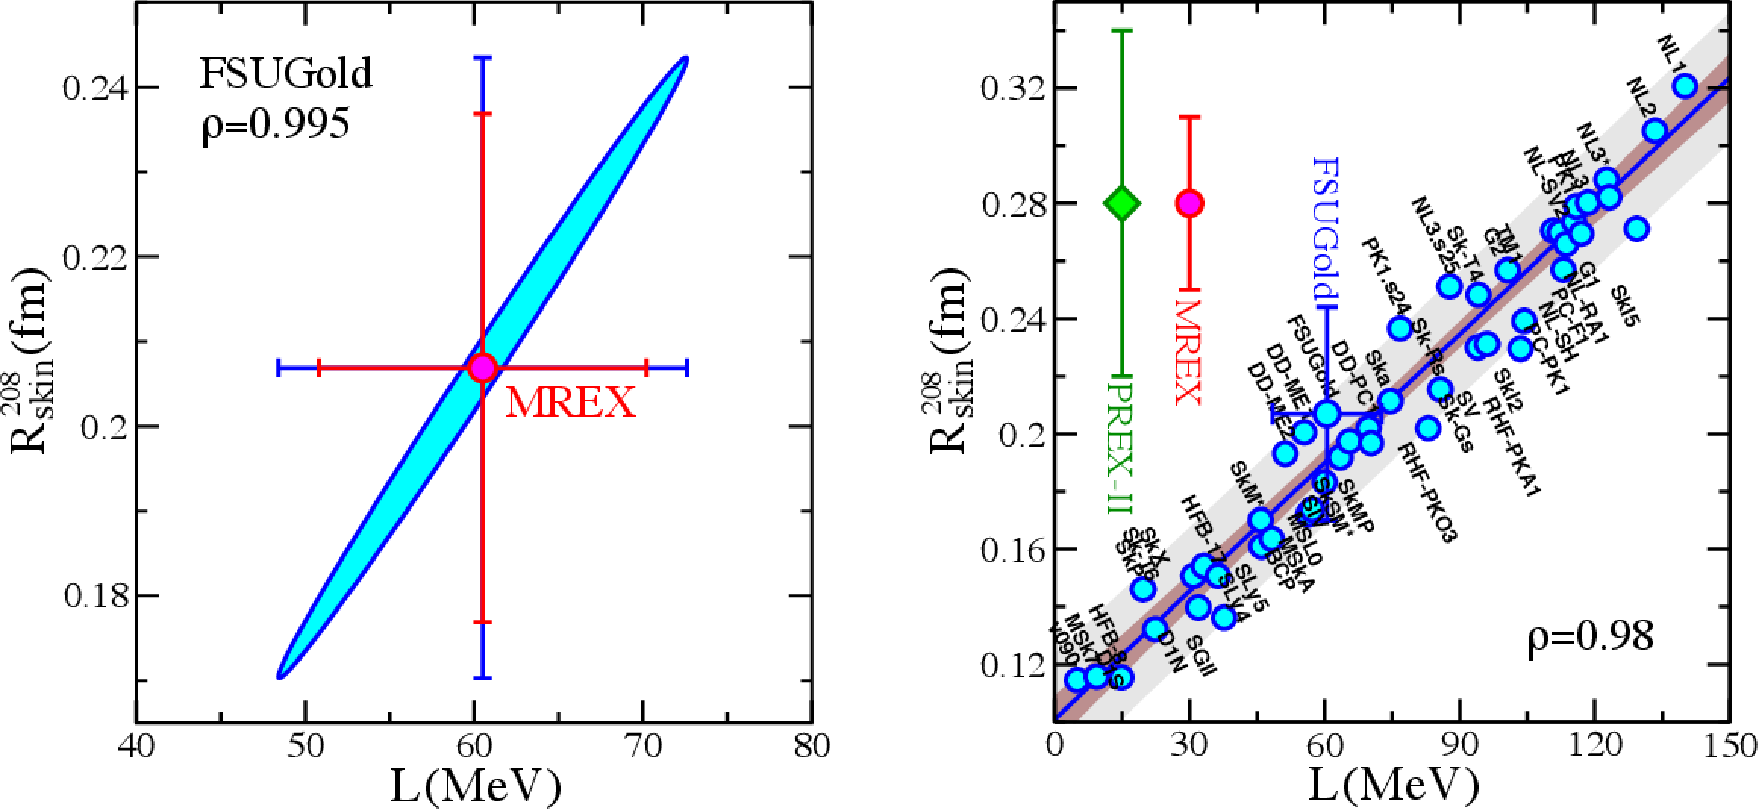
\includegraphics[width=0.75\textwidth]{Introduzione/LvsR.pdf}
 \caption{\textit{On the right} Neutron skin thickness of $^{208}Pb$ as a function of the slope of the symmetry energy $L$. The error bars represent $\pm \SI{0.06}{\femto \meter}$ and $\pm \SI{0.03}{\femto \meter}$ for the future experiments of PREX-II and MREX. Notice the different scale for x and y axis, a small uncertainty for the neutron skin measurement correspond to an higher uncertainty for the values of $L$. \textit{On the left} Covariance ellipse displaying the correlation between $L$ and the neutron skin thickness, for FSUGold model. The covariance $\rho$ is equal to 0.995.}
 \label{fig:LvsR}
 \end{figure}
 
A strong linear correlation is evident, and so it is clear that measuring the neutron skin is a promising way to measure $L$. 


  
\section{Parity-violating Scattering Experiment}

The parity violating electron scattering seems to be the most promising method in order to determine the neutron-skin thickness for $^{208}Pb$. The choice of lead is due to the significant neutron excess and stability of lead nuclei ($^{208}Pb$ is a double magic nucleus). The advantage of this method is that it is free from the many uncertainties associated to strong interaction. The main disadvantage is the necessity to accumulate large statistics, because the reaction are mediated by the weak interaction, that produce a smaller amplitude compared to electromagnetic and strong interaction. 
The parity violating scattering is high sensitive to the neutron density because, as mention above, the weak charge of the neutron is higher compared to the weak charge of the proton.
In this reaction, longitudinally polarized electrons are elastically scattered off a lead target. The important quantity to determine is the parity violating asymmetry $A_{PV}$, the difference in cross section between the scattering of right and left handed electrons. 

\begin{equation}
A_{PV} = \dfrac{\sigma_{R} - \sigma_{L}}{\sigma_{R} + \sigma_{L}}
\end{equation} 

The theoretical calculation of $A_{PV}$ concern the interference between the exchange of virtual $\gamma$ and $Z^{0}$. In the Born approximation $A_{PV}$ is directly proportional to the weak form factor, and it is given by the formula below:

\begin{equation}
A_{PV} \simeq \dfrac{G_{F} Q^{2}}{4 \pi \alpha} \cdot \dfrac{Q_{W} F_{W}(Q^{2})}{Z F_{ch}(Q^{2})}
\end{equation} 

$G_{F}$ is the Fermi constant, $Q^{2}$ is the transferred momentum, Z and $Q_{W}$ is the electric and weak charge of the nucleus. The Charged form factor of the lead nucleus is known with high accuracy (precision of 0.02 \%), so in this limit the only quantity that is unknown is $F_{W}(Q^{2})$. In the long wavelength approximation, the weak form factor at single value of momentum transfer is given by:

\begin{equation}
F_{W}(Q^{2}) = \frac{1}{Q_{W}} \int \rho_{W}(r) \dfrac{sin(Qr)}{Qr} d^{3}r = (1 - \frac{Q^{2}}{6} R^{2}_{W} + \frac{Q^{4}}{120}R^{4}_{W} + ...)  
\end{equation}

The form factor is normalized in such a way that $F_{W}(Q^{2} = 0) = 1$. The weak charge radius correspond to $R^{2}_{W} = -6 \frac{\partial F_{W}}{\partial Q^{2}}\Bigr|_{\substack{Q^{2} = 0}}$. Now it is clear that parity-violating experiment are a promising method to extract information about neutron density. The effort is represented by the small values of $A_{pv}$ asymmetry. Typical values are on the order of $1 \, ppm$ or less, for lead target. This requires high statistic to reduce the uncertainty of the measurement. 
In 2012 PREX collaboration measured for the first time through parity-violating experiment the neutron skin, the values is:

\begin{align*}
\delta r_{np} = 0.33^{+0.16}_{-0.18} \SI{}{\femto \meter}
\end{align*}

The error associated to this first measurement is not enough small to provide significant constraints on the values of $L$. Because of this, the MREX experiment has the objective of measuring the neutron radius of lead with a precision of $0.5 \%$  ($\pm \SI{0.03}{\femto \meter}$). This high precision is needed to decrease the uncertainty associated to L. For example, the left plot in \ref{fig:LvsR}, shows the correlation between the neutron skin thickness of $^{208}Pb$ and the slope of the symmetry energy as predicted by FSUGold model (\cite{Fattoyev_2011}). With a precision of $\pm \SI{0.03}{\femto \meter}$, $L$ is determined with $\pm \SI{12.1}{\mega \electronvolt}$. A new recent measurement, in 2019, measure the neutron skin thickness with a precision of 
$\delta r_{np} = 0.283 \pm 0.071 \SI{}{\femto \meter}$. With new measurement that will be performed in MESA accelerator by MREX, the precision will be improved further by a factor 2.

\subsection{Neutron Star Radius}

We mentioned that the slope of the symmetry energy $L$ is strongly correlated to the neutron skin thickness of $^{208}Pb$ and also to $R_{ns}$. We can go deeper in the discussion stating that the maximum neutron-star mass and radius are uniquely constrained by the E0S (\cite{Lindblom1992DeterminingTN}). The maximum mass depends on the energy density dependence of the Pressure, that must be high enough to oppose the gravitational collapse into a black hole. Moreover, stellar radii are strongly dominated by the pressure of degenerate nuclear matter near the saturation density.  
The connection between the radius of compact object and pressure is enclosed in Volkov-Oppenheimer equation; resolving the equation 
for a compact symmetric object gives the relation between radius and pressure $P_{c}$ at the center of the star (formal proof in \cite{LATTIMER_2007}).

\begin{equation}
R^{2} = \dfrac{3}{8\pi \rho} \dfrac{1 - (\rho + P_{c})^{2}}{(\rho + 3 P_{c})^{2}}
\end{equation}

But the pressure $P_{c}$ is, in large part, determined by the symmetry energy of the equation of state, so there should be a strong correlation between $L$ and the neutron star radius $R_{ns}$. In the end, different theoretical models \cite{PhysRevLett.95.122501} confirms the connection between $L$ and $R_{ns}$, for example we show the covariance ellipses predicted by FSUGold model between the slope of the symmetry energy $L$ and the stellar radii:

\begin{figure}[hbtp]
\centering
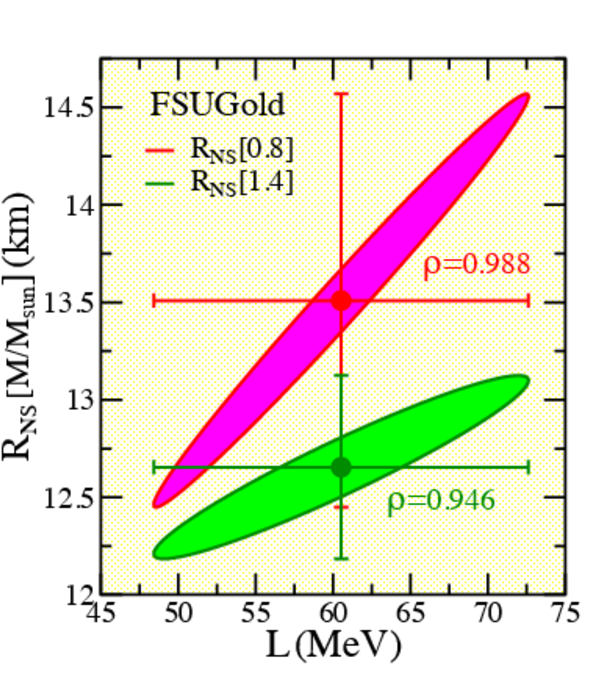
\includegraphics[width = 0.5\textwidth]{Introduzione/LvsRns.pdf}
\caption{Covariance ellipses between slope of the symmetry energy and stellar radii, for $0.8$ and $1.4$ solar masses, predicted by the relativistic density model FSUGold.}
\end{figure}

From these consideration, astronomical observation of Mass and radii of neutron stars represents important constrain on the EOS, and are valuable for understanding the behaviour and physics of the atomic nuclei.
Astronomical observations of the neutron star radius rely traditionally on photometric measurements, assuming that thermal emission of light from the surface follow a blackbody spectrum at uniform temperature. These measurement are affected by systematic uncertainties that are typically of a couple of kilometers.
However, the situation is rapidly changed with the beginning of the gravitational wave detection. The first observation of the binary neutron star merger by the LIGO-Virgo collaboration opened a new path to measure the neutron-stars radius \cite{LIGOScientific:2017vwq}. In fact, the gravitational wave generated by the merging of two neutron stars depends on a property called tidal deformability; this parameters described the tendency of neutron star to deform in response of the gravitational field of its companion star. This parameters $\Lambda$, is highly sensitive to the ratio of the stellar radius to the Schwarzschild radius:

\begin{equation}
\Lambda = \frac{2}{3} k_{2} \big( \dfrac{c^{2} R_{NS}}{GM} \big)^{5}
\end{equation}

In this expression, M and $R_{NS}$ are the neutron star mass and radius, and $k_{2}$ is the second tidal Love number \cite{Binnington:2009bb}, which is computed from the quadrupole component of the gravitational field induced by the companion. From the first detection, an upper limit of $R_{NS}^{1.4} < \SI{13.76}{\kilo \meter}$ was placed on the radius of a neutron star with a $1.4$ solar masses. Because of the strong correlation between $R_{NS}$, $L$ and $\delta r_{np}$, this is a indirect constrain on the neutron skin thickness of $^{208}Pb$. An upper limit of $\delta r_{np} < \SI{0.25}{\femto \meter}$ was obtained. This limits is not consistent with the larger values measured by PREX collaboration; this can suggest that the symmetry energy, for slightly higher density as in neutron stars, decreases, respect the typical density found in atomic nuclei. This increment and decrement may be a proof of the presence of phase transition in the interior of neutron stars.


\section{Transverse Asymmetry}

\commento{Here we have to introduce the aim of this thesis: the transverse asymmetry is a source of background for the parity-violating experiments. Furthermore the theory is not working well for some nuclei ($^{208}Pb$), so mention PREX paper about the last measurement on carbon and lead, the problem that they measure $0$ transverse asymmetry.}

The parity-violating scattering has numerous advantages for extracting the neutron-skin thickness of nuclei. However, the asymmetry to measure is rather small. The important effort is to reduce at most possible systematic effects that can alter the result of the measurement. One of the principal source of background for the measurement of $A_{PV}$ is a different process that concerns transverse polarized electrons. The different polarization of the electrons produce an asymmetry that is called beam normal single spin asymmetry, or transverse asymmetry $A_{n}$. Because such asymmetries are typically one order higher that the parity-violating ones, a small normal component of the beam polarization during parity-violating experiment can produce a systematic effect that alter the final result. The subject of this thesis is the measurement of transverse asymmetry $A_{n}$ for carbon target, performed at MAMI, the Mainz microton accelerator. The choice of carbon target is due to the fact that the transverse asymmetry for $^{12}C$ is well known and already measured at MAMI; the expected asymmetry is roughly $20 \, ppm$ , thus it is particularly suited for a commissioning of the new experimental setup. In this section don't introduce physics of this process, that will be extensively treated in the next chapter. However, we mention that such measurement are challenging because they require calculation of box diagrams with intermediate excited states \cite{Gorchtein_2008}.
After the determination on $A_{n}$ for $^{12}C$, the next step of the MREX experiment will be the determination of the \transv for $^{208}Pb$. As already mentioned, this is mandatory to constrain the systematic effects of PV experiment. However, it is also interesting because for last measurement performed by PREX \cite{HAPPEX:2012fud} the \transv for $^{208}Pb$ target is compatible with zero, and this is in striking disagreement with the theoretical predictions. 
